\documentclass[runningheads]{llncs}
\usepackage[utf8]{inputenc}
\usepackage[spanish]{babel}
\usepackage{dirtytalk}
\usepackage{graphicx}
\usepackage[section]{placeins}
\usepackage{float}
\usepackage{caption}

\begin{document}

\title{Minado de datos mediante Orange.}
\author{Hugo Pérez Fernández.  \email{UO250708@uniovi.es}
\institute{Sistemas de Información para la Web. Grado en Ingeniería del Software. EII. 
Universidad de Oviedo. Campus de los Catalanes. Oviedo}}
\maketitle
    
\section{Introducción}

En este documento se realizará un estudio sobre un dataset, que contiene una linea de tiempo con 15 noticias y si la bolsa 
subió o bajó, para realizar un modelo de predicción de la subida o bajada de la bolsa. Para ellos nos apoyaremos en la 
herramienta de software Orange, que nos permitirá el minado de datos en el dataset y la realizacion de diferentes modelos 
supervisados y no supervisados.

\section{Decisiones}

Los primeros pasos en el estudio del dataset han sido los mismos en todos los casos:

\begin{enumerate}
    \item \textbf{CSV File Import}: Leer el archivo que contiene el dataset dado.
    \item \textbf{Corpus}: Se genera un corpus a partir del dataset dado en el que los documentos serán cada una de las
        noticias.
    \item \textbf{Process Text}: Se procesa el texto de modo que se pasa todo a minúsculas, se tokeniza para quedarnos con palabra, 
        y se filtra de manera que se eliminen las palabras vacias del inglés, puesto que las noticias estan en ese idioma y las de 
        una lista negra generada por mi que se encuentra en el directorio del proyecto,está lista negra se ha obtinido de la obserbación de 
        de un Word Cloud, finalmente se le aplica una expresión regular para eliminar caracteres especiales y el caracter b' y b" 
        presentes en el dataset.
\end{enumerate}

Posteriormente se ha decidido afrontar el problema de dos formas, en el primer caso se usa la Bag of Words, generada con la siguiente configuración; 
La frecuencia de términos se calcula mediante un contador, para la frecuencia del documento se usa la estrategia IDF y para la regularizacion una suma 
de elementos directamente para realizar los modelos, y en la segunda forma, tras construir la Bag of Words, se realiza un modelado de Topics, en el que se 
generan 10 tops de terminos de modo que al corpus se le añade la similitud a estos para cada documento.

\begin{figure}[H]
    \center
    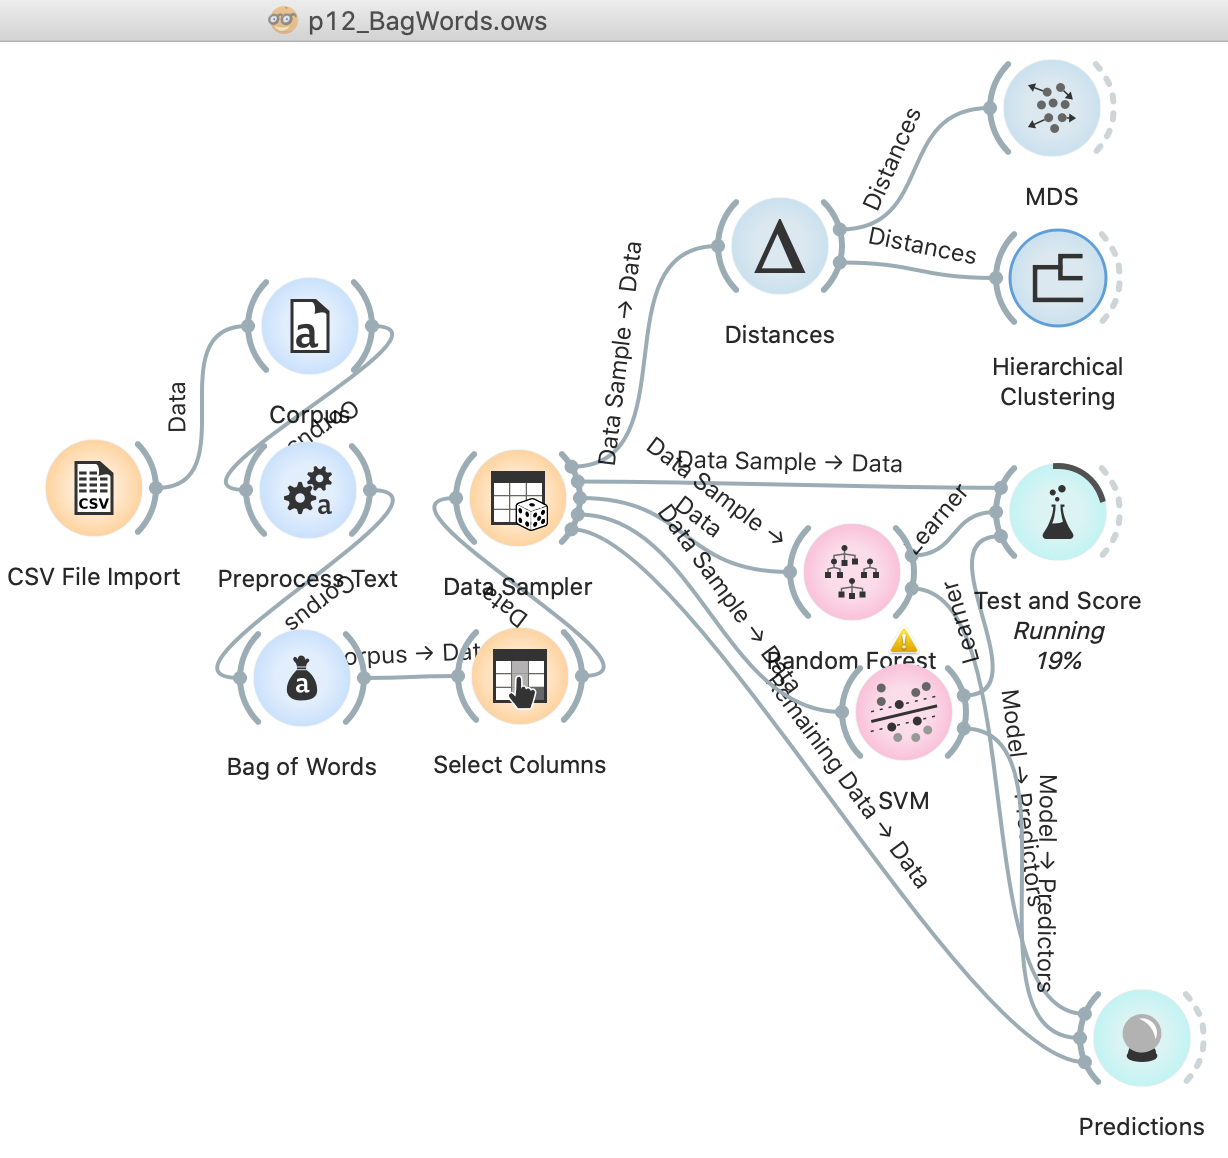
\includegraphics[width=1\linewidth]{resources/BagWordsFlow.png}
    \caption{ Flujo Orange con Bag of Words.}
    \label{fig:1}
\end{figure}
\begin{figure}[H]
    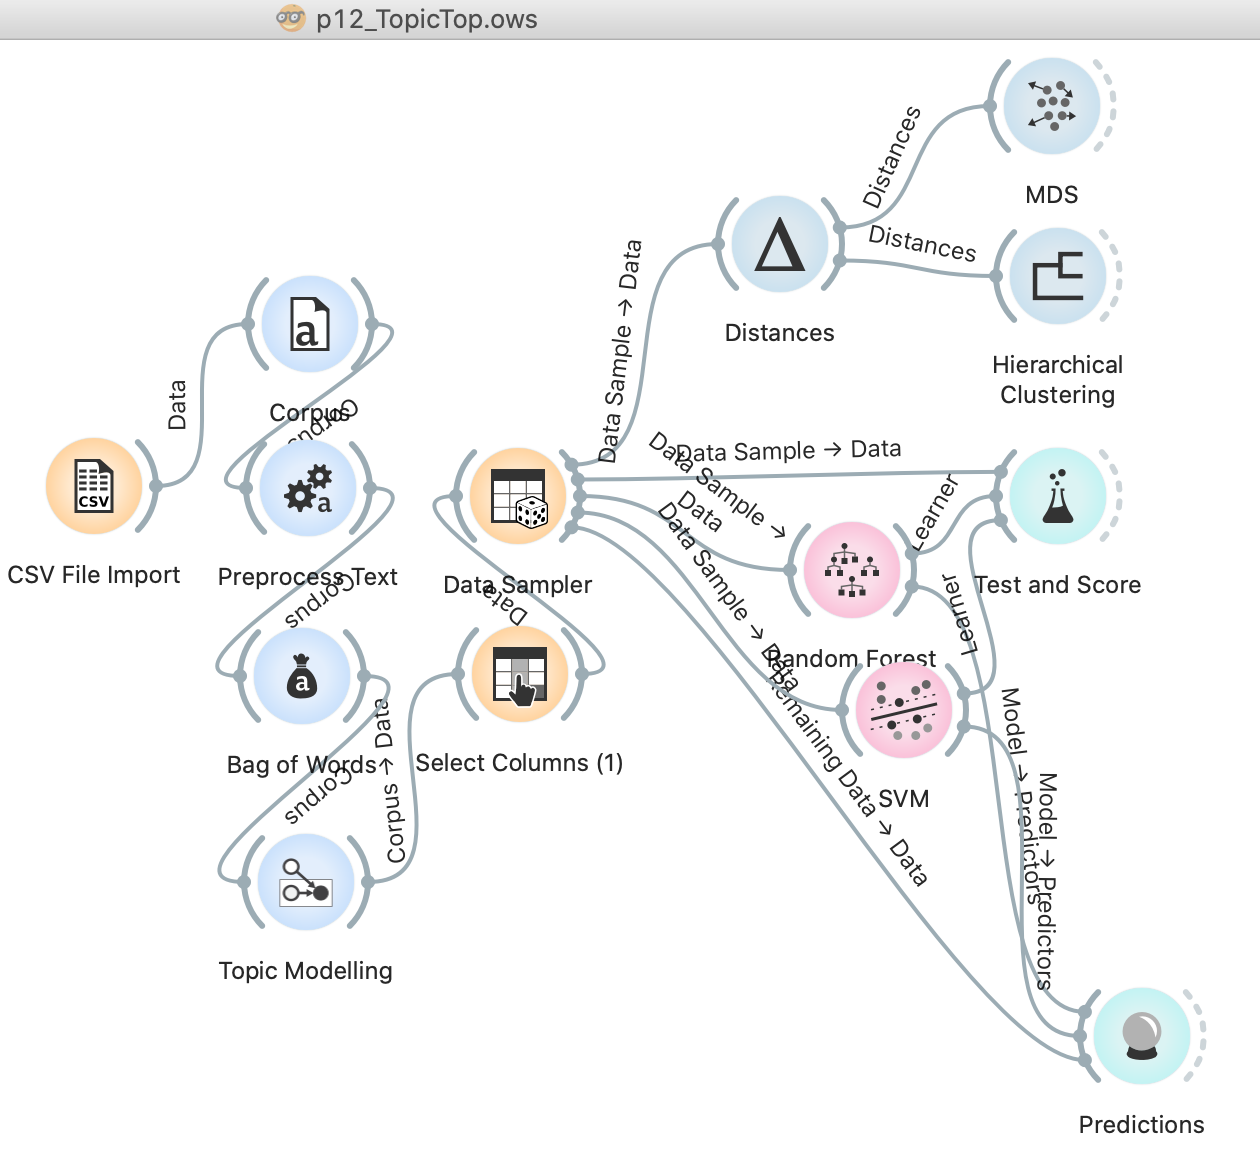
\includegraphics[width=1\linewidth]{resources/TopicTopFlow.png}
    \caption{  Orange con Bag of Words y Top Topics.}
    \label{fig:2}
\end{figure}

Esta decisión se ha tomado puesto que puede que la notícia que haya presente en cada entrada del dataset no sea verdaderamente 
importante pero si los topics que estas generan, de manera que si en las noticias presentes se obtiene un topic de guerra quizas 
podemos aprender que si se da este hecho la bolsa baje o suba. De igual modo otra aproximación que se prodría aplicar es usar 
algún sistema de deteccion de emociones para que dadas estas noticias se interpole el estado de animo que podrían producir de 
modo que puede que se encuentre algun patron entre el estado de ánimo y la subida o bajada de la bolsa, pero en este caso no 
es posible puesto que Orange no contiene ningun nodo que lo ofrezca.


Ahora se realizarán los ultimos pasos para la preparacion de los datasets:

\begin{enumerate}
    \item \textbf{Select Column}: Se selecciona la clase que se usará para el aprendizaje supervisado, y ademas se puedes seleccionar
    los atributos que se usaran para generar los modelos en el caso de que no se quieran usar todos.
    \item \textbf{Data Sampler}: Se particiona el dataset en 75\% para aprendizaje y validación y 25\% para el posterior testeo del modelo.
\end{enumerate}

Tras la preración de los datos que se ha explicado anteriormente se han probado diferentes casos de aprendizaje que se pueden dividir en función de 
si el aprendizaje para el modelo ha sido supervisado o no supervisado.

\subsection{No supervisado}

Para este caso se ha elejido el aprendizaje MDS y Clusterización Jerarquica, con un sistemas de calculo de distancias que aplica el coseno,
como se muestra a continuacion los resultados no son buenos puesto que en ambos casos la división no es clara y son necesarias demasiadas agrupaciones.

\begin{figure}[H]
    \center
    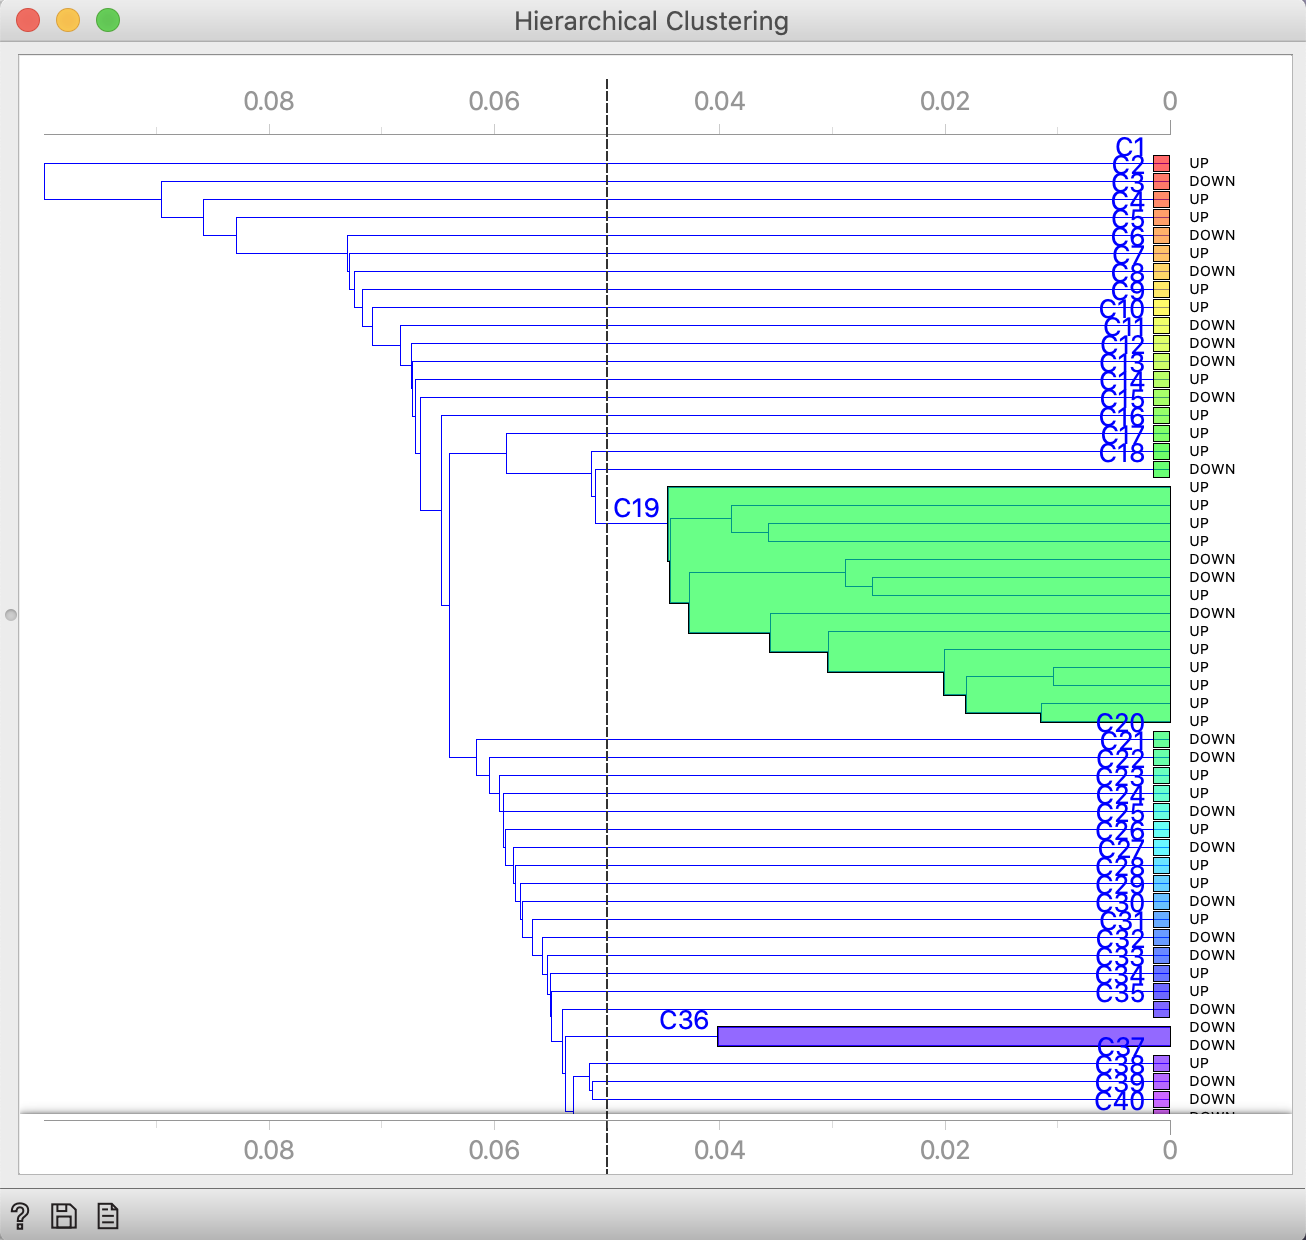
\includegraphics[width=1\linewidth]{resources/HierarchicalClustering.png}
    \caption{ Clusterizacion jerarquica del DataSet.}
    \label{fig:3}
\end{figure}
\begin{figure}[H]
    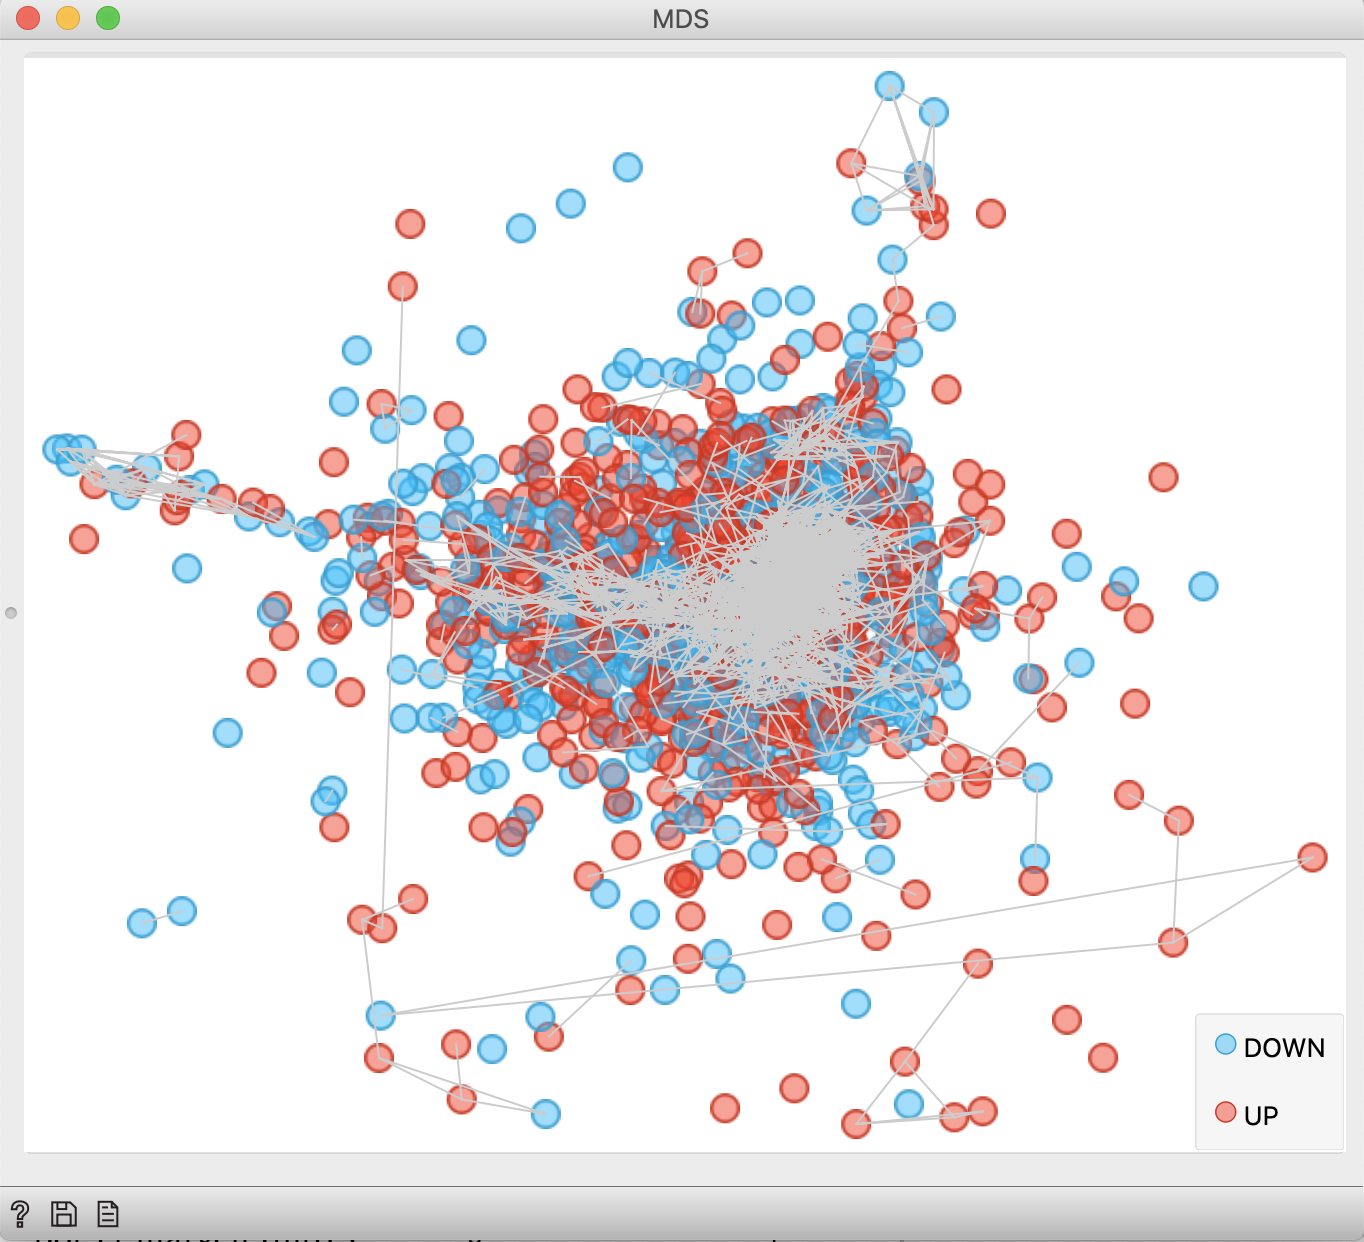
\includegraphics[width=1\linewidth]{resources/MDS.png}
    \caption{ MDS del DataSet.}
    \label{fig:4}
\end{figure}

\subsection{Supervisada}

Para este caso se ha elejido el aprendizaje Random Forest y SVM con las siguintes configuraciones:

\begin{itemize}
    \item \textbf{Random Forest}:
    \begin{itemize}
        \item Configuraciones predefinidas.
    \end{itemize}
    \item \textbf{SVM}:
    \begin{itemize}
        \item $C = 0.3$
        \item $\varepsilon = 0.1$
        \item El resto de configuraciones predefinidas.
    \end{itemize}
\end{itemize}

\section{Analisis de Resultados}

A continuación se mostraran los resultados obtenidos con los dos flujos de trabajo en orange para los modelos de aprendizaje supervisado.

\begin{figure}[H]
    \center
    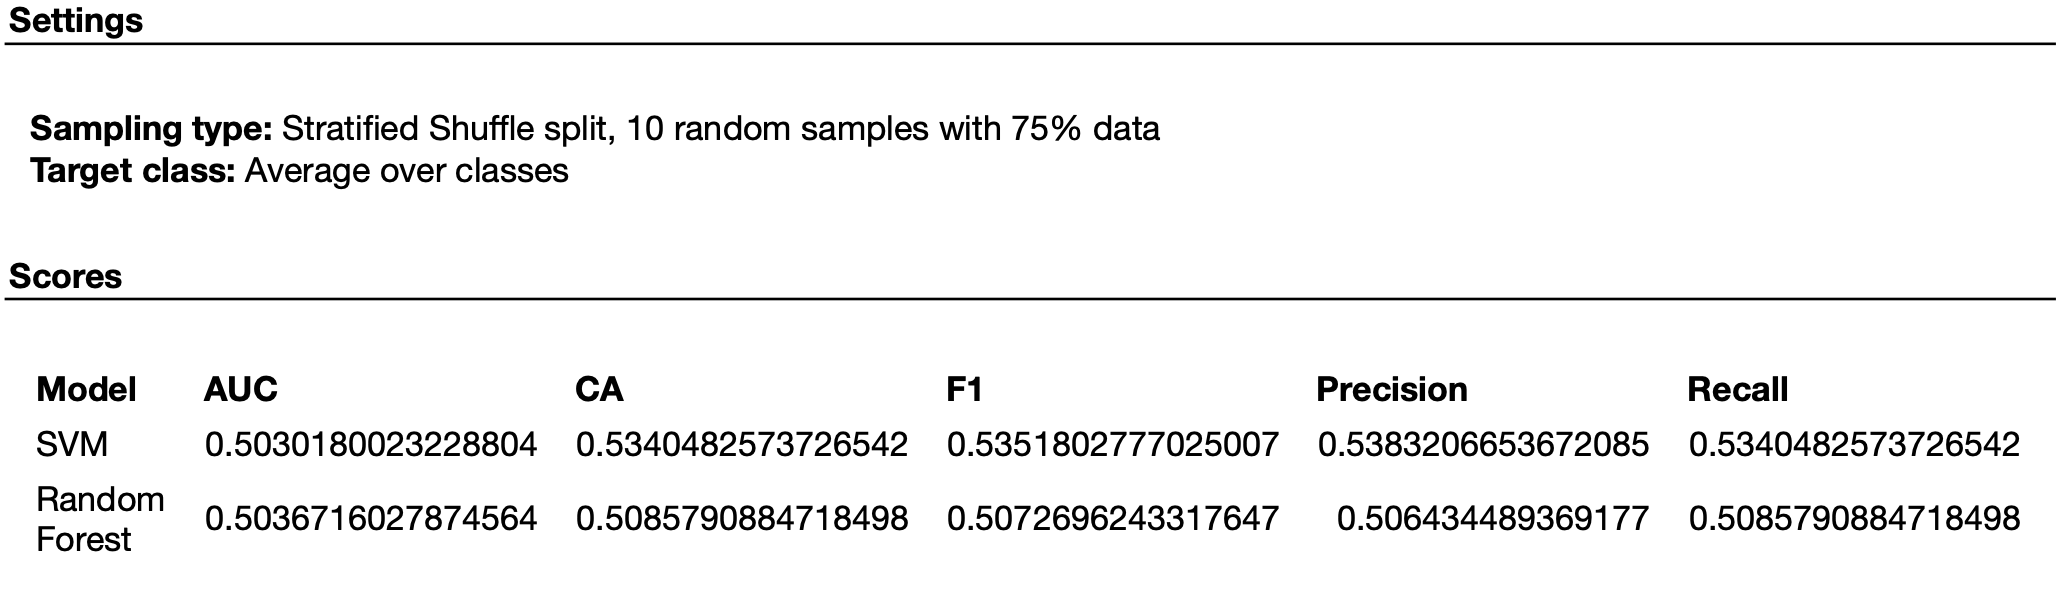
\includegraphics[width=1\linewidth]{resources/ReportTopTopic.png}
    \caption{ Reporte de los modelos del flujo con Bag of Words y Top de Topics.}
    \label{fig:5}
\end{figure}
\begin{figure}[H]
    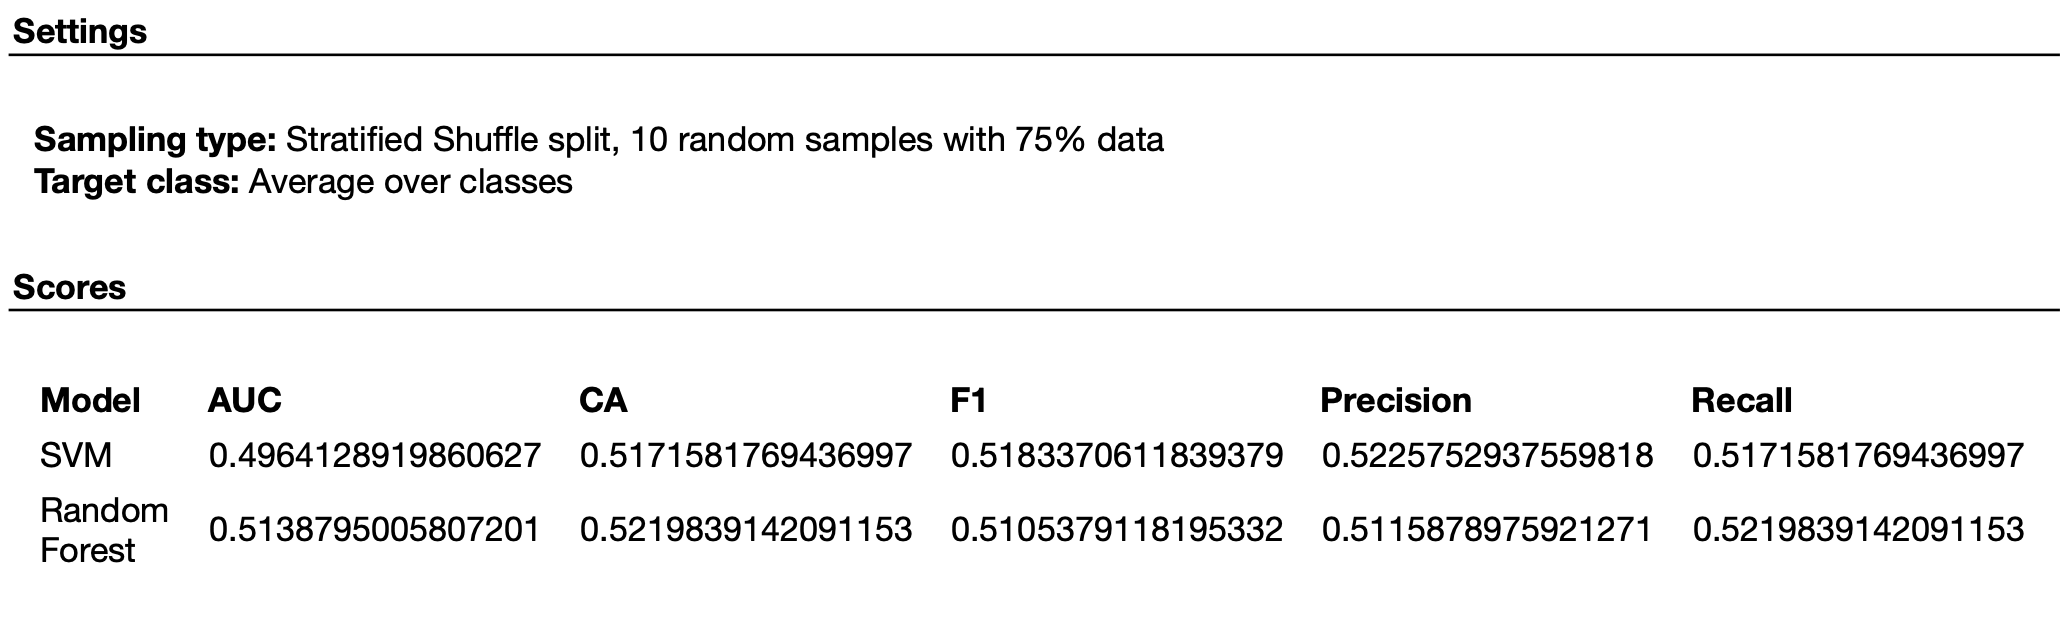
\includegraphics[width=1\linewidth]{resources/ReportBagWords.png}
    \caption{ Reporte de los modelos del flujo con Bag of Words.}
    \label{fig:6}
\end{figure}

Como se puede observar en las imágenes anteriores en ninguno de los casos los modelos predictivos difieren en gran medida 
de lo que se conseguiría lanzando una moneda, por lo que podemos decir que se trata de malos modelos.

Si cabe destacar que el modelo generado con SVM mejora en cierta medida la de Random Forest y ademas hay que mencionar que 
en el caso del flujo de orange en el que se usan los Tops de Topics el tiempo de generación de los modelos es mucho menor 
que en el flujo en el que solo se realiza la Bag of Words de modo que al menos experimetar se vulve menos tedioso y además 
los restuados de precesión son mejores al usar los topics y no las Bag of Words.

\end{document}